The Standard Model (SM) of particle physics is a highly successful, commonly accepted description of the fundamental particles and their interactions and at the same time subject to several shortcomings, motivating the search for signs of new phenomena beyond its scope. In this chapter a short overview of the SM and its shortcoming is given. Supersymmetry is presented as an attractive candidate for the extension of the SM and the phenomenological consequences of its existence relevant to this analysis are discussed. 
\section{The Standard Model of particle physics}
The SM describes the fundamental particles in the framework of a renormalizable quantum field theory, in which each particle is represented by one quantum field~\cite{Glashow1961579,Salam1964168,PhysRevLett.19.1264,PhysRevD.5.1412}. Two fundamental classes of particles are distinguished, bosons with integer and fermions with half-integer spin. 

The fermions are in turn classified as quarks or leptons. The different types of quarks and leptons are known as ``flavours''. There are six quark flavours, called up, down, strange, charm, bottom and top, and three electrically charged lepton flavours, electron ($e$), muon ($\mu$) and tau ($\tau$). The electrically neutral leptons, called neutrinos ($\nu$), are assigned the names of the charged lepton of their generation. Of these there are three, each consisting of a charged lepton and the corresponding neutral neutrino and two quarks. Of the latter one is up-type with an electric charge of $+\frac{2}{3}e$ and the other is down-type with charge $-\frac{1}{3}e$. The particle content of the fermionic sector of the SM is summarized in Table~\ref{tab:fermions}.

\begin{table}
\centering
 \renewcommand{\arraystretch}{1.3}
\caption{Fermions in the Standard Model. All masses are taken from~\cite{PDG} and quoted without their uncertainties.}
\label{tab:fermions}
\begin{tabular}{l|c c c | c c c }
  & \multicolumn{3}{c|}{Leptons} & \multicolumn{3}{c}{Quarks} \\
    & flavour & charge [$e$] & mass [GeV] & flavour & charge [$e$] & mass [GeV] \\
    \hline
  \multirow{2}{*}{1$^{\mathrm{st}}$ generation} & $e$ & -1 & 511$\cdot$10$^{\mathrm{-6}}$ &  down & $-\frac{1}{3}$ & 2.3$\cdot$10$^{-3}$ \\
 												& $\nu_e$ & 0 & $<$2$\cdot$10$^{\mathrm{-9}}$ &  up & $+\frac{2}{3}$ & 4.8$\cdot$10$^{-3}$  \\
 												\hline
  \multirow{2}{*}{2$^{\mathrm{nd}}$ generation} & $\mu$ & -1  & 105.7$\cdot$10$^{\mathrm{-3}}$ & strange & $-\frac{1}{3}$ & 95$\cdot$10$^{-3}$ \\
 												& $\nu_{\mu}$ & 0 & $<$2$\cdot$10$^{\mathrm{-9}}$ & charm & $+\frac{2}{3}$ & 1.3 \\
 												\hline
  \multirow{2}{*}{3$^{\mathrm{rd}}$ generation} & $\tau$ & -1 & 1.8 & bottom & $-\frac{1}{3}$ & 4.2\\
 												& $\nu_{\tau}$ & 0 & $<$2$\cdot$10$^{\mathrm{-9}}$ & top & $+\frac{2}{3}$ & 173.2 \\ 												
 
 
\end{tabular}

\end{table}

Of the four fundamental forces, the electromagnetic, weak, strong and gravitational forces, the first three are described within the SM. Each of these forces is mediated by spin-1 gauge bosons. In the case of the electromagnetic force this is the massless photon, which couples to the electric charge of particles. The weak force is mediated by three massive bosons, the W$^{\pm}$ ($m_{\mathrm{W}} = \unit{80.4}{\giga\electronvolt}$) and the Z$^{0}$ ($m_{\mathrm{Z}} = \unit{91.2}{\giga\electronvolt}$), coupling to the weak charge. The charge of the strong force is called colour, to which 8 massless gluon couple. Of all fermions, only the quarks carry colour and participate in the strong interaction. 

The group structure of the SM is $SU(3)_C \times SU(2)_L \times U(1)_Y$. The $SU(3)_C$, with $C$ representing the colour charge, is the gauge group associated with the strong interaction. From the non-abelian structure of this group follows the presence of three and four gluon interactions in the SM~\cite{Pich:2007vu}. Therefore the strong interaction increases with distance, leading coloured particles to only exist in bound states. So far the existence of two- and three-quark states (mesons and baryons) has been established. 

The subgroup $SU(2)_L \times U(1)_Y$ describes the unification of weak and electromagnetic interaction in the electroweak theory. The index $L$ indicates that the weak isospin $T$ couples only to left-handed particles and $Y$ is the weak hypercharge. The $SU(3)_L$ introduces three vector fields, of which two mix to the observed W$^{\pm}$ = $\frac{1}{\sqrt{2}}(W^1\mp iW^2)$. The remaining neutral W$^3$ mixes with the B$^0$ arising from the $U(1)_Y$ group to form the photon and Z boson~\cite{HalzenMartin}.

To give masses to the particles, the Higgs mechanism is introduced~\cite{PhysRevLett.13.508,PhysRevLett.13.321,PhysRevLett.13.585}. It postulates a complex scalar doublet that spontaneously breaks the $SU(2)_L$ gauge symmetry, allowing to give masses to the electro-weak gauge bosons while the $U(1)_Y$ remains unbroken and the photon massless. Fermions acquire mass through a Yukawa coupling to the Higgs field. The Higgs mechanism results in the presence of a massive neutral scalar boson. The discovery of such a particle with a mass of $\unit{125}{\giga\electronvolt}$ by the CMS and ATLAS collaborations at the LHC in 2012~\cite{Chatrchyan:2012ufa,Aad:2012tfa} and the good agreement of its properties with the prediction of the SM~\cite{Khachatryan:2014jba} provides evidence for the validity of this theory.   

\subsection*{Shortcomings of the Standard Model}
The discovery of the Higgs boson is a large success for the SM, and only the last in a long series of experimental results vindicating the decades old theory. However, for a long time also the shortcomings of the SM have been known. Here only those most relevant to the motivation of Supersymmetry are discussed.

\subsubsection*{Higgs mass and naturalness}
One of the most pressing issues is directly related to the Higgs boson and its mass. Quantum loop corrections to the bare Higgs mass change the observable mass of the particle. For example the coupling to a fermion with coupling strength $\lambda_f$ results in a correction of
\begin{equation}
\Delta m_{H}^2 = -\frac{|\lambda_f^2|}{8\pi^2}\Lambda_{UV}^2 + ...,
\end{equation}
where $\Lambda_{UV}$ represents the energy scale up to which the SM is valid as an effective theory, i.e. the scale at which new physics will be appear. This is expected to be the Planck scale $M_P = (8\pi G_{\mathrm{Newton}})^{-\frac{1}{2}} = \unit{2.4\times 10^{18}}{\giga\electronvolt}$, where effects of gravity become important at the quantum level. Therefore the loop corrections are of enormous magnitude and have to precisely cancel a bare Higgs mass of similar magnitude to a degree that leads to an observable Higgs mass at the electroweak breaking scale. This required fine-tuning is known as the  $\textit{hierachy problem}$ and is considered to be unnatural and motivates the presence of new physics at the TeV scale.

\subsubsection*{Astrophysical Observations}
Astrophysical observation have been suggesting the presence of non-visible forms of matter, for example from the motion of galaxy clusters or galaxy rotation curves. The most precise measurements of the energy content of the universe come from observations of the cosmic microwave background~\cite{Adam:2015rua}. The contribution of ordinary matter is only about 4.9\%, while an unidentified dark matter, interacting only gravitational and possibly weakly, accounts for about 25.9\% (the remaining 69.2\% are attributed to dark energy). The SM does not provide any candidate for a dark matter particle, after neutrinos have been disfavoured by structure formation in the early universe. Possible candidates would be so far undiscovered weakly interacting massive particles with masses in the order $\mathcal{O}(\unit{100}{\giga\electronvolt}$), which would required an extension of the SM. 

\subsection*{Unification of forces}
In the past the increasingly deeper insights into the workings of nature have often allowed to find unified theoretical frameworks to describe different physical phenomena, for example the unification of electric and magnetic force into electromagnetism or its further unification with the weak force into the electroweak theory discussed above. Therefore a further unification with the strong force into a grand unified theory (GUT) at higher energy scales is hoped for. However, as shown by the dashed lines in Figure~\ref{fit:unification}, the running couplings of the three forces do not meet at any energy scale in the SM, excluding a unification inside the existing theoretical framework. As already indicated in the Figure, this could be remedied by extension of the SM such as Supersymmetry, where the introduction of new particles at the TeV scale changes the running of the couplings.
\begin{figure}
\centering
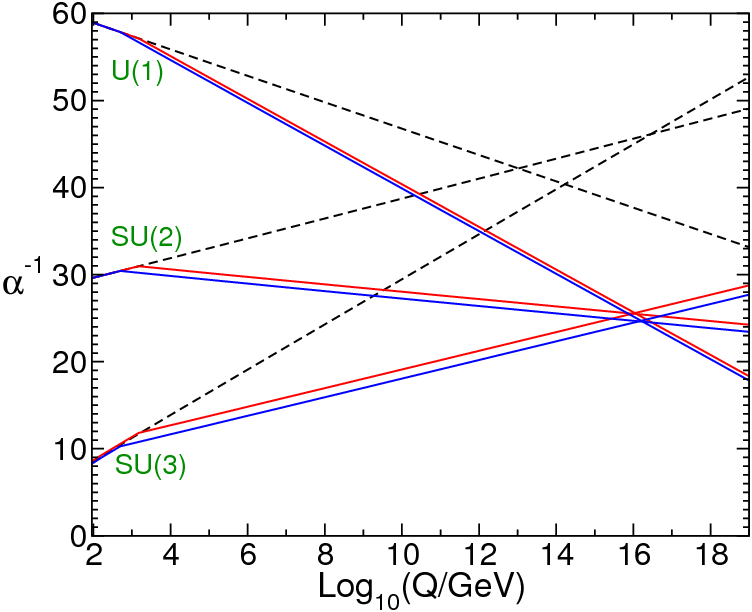
\includegraphics[scale=0.35]{plots/THEO/unification.png}
\caption{Running of the coupling of the electromagnetic, weak and strong force in the Standard Model (dashed lines) and Supersymmetry (red and blue lines).}
\label{fit:unification}
\end{figure}
\section{Supersymmetry}
Of the many proposed extension of the SM, Supersymmetry (SUSY) has been considered to be the most attractive in the last decades. It postulates the existence of a fermion partner to every SM boson and vice versa. This promises a solution to the naturalness problem of the Higgs boson mass and might also lead to a unification of forces and in certain models offer candidates for the dark matter particle. In the following a short description of the theoretical framework, based on~\cite{Martin:1997ns}, is given before the phenomenological consequences and the experimental signatures relevant to this analysis are discussed.
\subsection{Theoretical foundation}
Supersymmetry introduces a symmetry between bosons and fermions. In the minimal supersymmetric extension of the Standard Model (MSSM), one $\textit{superpartner}$ is assigned to each SM particle which has the same quantum numbers except for the spin, which differs by $\frac{1}{2}$. The designated names of the new supersymmetric particles ($\textit{sparticles}$) are derived by adding the prefix $\textit{s-}$ to all fermion partners and the postfix $\textit{-ino}$ to all boson partners. The same scheme holds also for categories of particles, so that $\textit{sleptons}$ and $\textit{squarks}$ are the partners of leptons and quarks and make up the $\textit{sfermions}$ while the $\textit{gauginos}$ are the partners of the gauge bosons. 

The SM Higgs sector has to extended two complex scalar doublets to give masses to the particles
\begin{eqnarray}
H_1 = \colvec{2}{H_1^0}{H_1^-}, & &  H_2 = \colvec{2}{H_2^0}{H_1^+}.
\end{eqnarray}
Here $H_1$ gives mass to down-type quarks and leptons while $H_2$ gives mass to up-type quarks. To these four Higgs states $\textit{higgsinos}$ are introduced as superpartners. In the spontaneous symmetry breaking eight degrees of freedom appear instead of four because of the presence of the second doublet. Three are used to give mass to the W and Z bosons, leaving five massive bosons. Therefore SUSY results in an extended Higgs sectors with two neutral scalars, $h^0$ and $H^0$, one neutral pseudoscalar $A^0$, and two charged scalars $H^{\pm}$. By convention $h^0$ is the lighter of the two scalars and commonly identified with the observed Higgs boson. 

The higgsinos and gauginos mix two eight mass eigenstates, the charginos $\chi^{\pm}_1$ and $\chi^{\pm}_2$ and the neutralinos $\chi^0_1$,$\chi^0_2$,$\chi^0_3$, and $\chi^0_4$. The additional particle content introduced in the MSSM is summarized in Table~\ref{tab:MSSM}.

\begin{table}
\centering
 \renewcommand{\arraystretch}{1.3}
\caption{Additional particle content of the MSSM.}
\label{tab:MSSM}
\begin{tabular}{c|c|c|c}
particle & gauge eigenstates  & mass eigenstates & spin   \\
\hline
\multicolumn{4}{c}{Standard Model} \\
\hline
Higgs bosons & $H_1^0$, $H_1^{-}$, $H_2^0$, $H_2^+$ & $h^0$, $H^0$, $A^0$, $H^{\pm}$ & 0 \\
\hline
\multicolumn{4}{c}{Supersymmetry} \\
\hline
squarks & $\tilde{q}$ & $\tilde{q}$ & 0 \\
sleptons & $\tilde{l}$ & $\tilde{l}$ & 0 \\
 gluino & $\tilde{g}$ & $\tilde{g}$ & 0 \\
neutralinos & $\tilde{W}^0$, $\tilde{B}^0$, $\tilde{H}_1^0$, $\tilde{H}_2^0$ & $\chi^0_1$,$\chi^0_2$,$\chi^0_3$, $\chi^0_4$ & $\frac{1}{2}$\\
charginos & $\tilde{W}^+$, $\tilde{W}^-$, $\tilde{H}_1^-$, $\tilde{H}_2^+$ & $\chi^{\pm}_1$,$\chi^{\pm}_2$ & $\frac{1}{2}$ \\ 
\end{tabular}
\end{table} 

If such a model would be realized it would alleviate the hierachy problem because the contributions of the superpartners to the quantum loop corrections to the Higgs mass have opposite sign than those of the SM particles, cancelling the dependency on the cutoff parameter $\Lambda_{UV}$. However, as no superpartners have been discovered so far, SUSY must be a broken symmetry and they can't have the same mass as the corresponding SM particles but must be heavier. Therefore the cancellation of contributions to the Higgs boson mass becomes imperfect. To prevent the need for fine-tuning, sparticle masses are expected to be at the TeV scale. Especially the top squark mass must to rather small as the top quark is the heaviest SM particle and contributes dominantly to the loop corrections. 

SUSY introduces lepton- and baryonnumber violating couplings, which would allow for rapid proton decay, in contradiction to its extremely long lifetime. To keep the proton stable, the quantum number R-parity
\begin{equation}
R_P = (-1)^{3(B-L)+2s}
\end{equation} 
is introduced, with B, L and s being the baryon number, lepton number and spin of the particle. It is +1 for all SM particles and -1 for all SUSY particles. If R-parity is conserved, SUSY particles can only produced in even number and the lightest supersymmetric particle (LSP) must be stable. In many SUSY models the LSP is the lightest neutralino $\chi^0_1$, providing a possible dark matter candidate. 


\subsection{Dilepton mass edges in SUSY}
The multitude of superpartners offer a rich variety of experimental to be observed at hadron colliders such as the LHC. The discussion here focusses on R-parity conserving models. In Figure~\ref{fig:SUSYXSecs}, the pair production cross section for different combinations of SUSY particles in proton-proton collision at a centre-of-mass energy of $\unit{\sqrt{s}=8}{\tera\electronvolt}$ is shown. It can be seen that the production of squarks and/or gluinos via the strong force is the dominant production mode. It therefore seems natural to focus on these events in the search for SUSY.
\begin{figure}
\centering
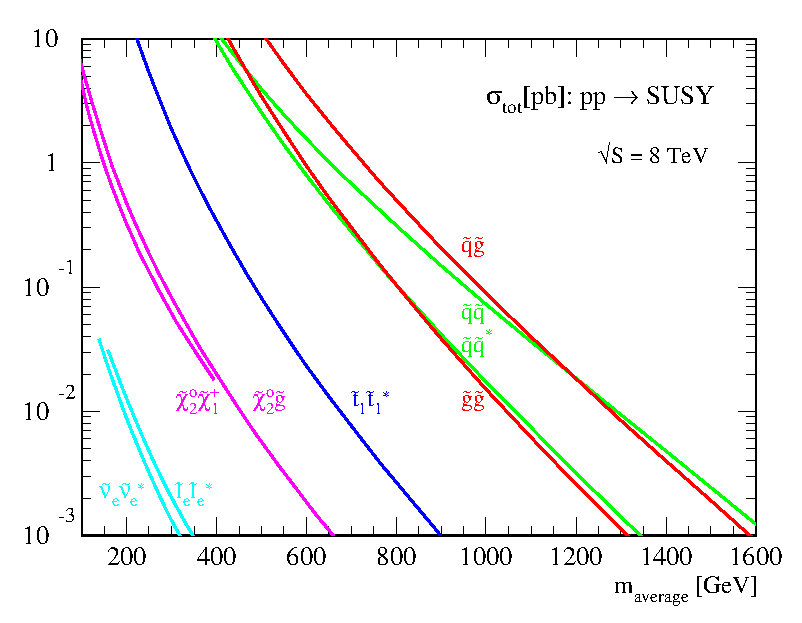
\includegraphics[scale=0.6]{plots/THEO/prospino_lhc8.eps}
\caption{Cross sections for pair production of SUSY particles in proton-proton collision at $\sqrt{s} = \unit{8}{\tera\electronvolt}$ as a function of the average mass of the produced pair~\cite{ProspinoPlot,Beenakker:1999xh,Beenakker:1997ut,bib-nlo-nll-01}.}
\label{fig:SUSYXSecs}
\end{figure}

The experimental signature of SUSY are cascades of decays of the initially produced particles into the LSP under emission of several SM particles. In the case of strong production, at least two quarks or gluons are produced in the first decays of the two decay chains in the events. These will hadronize into jets. Often even more jets are produced in the decays chains, making high jet multiplicities and large amounts of hadronic energy typical signatures of SUSY. The LSP is stable and will leave the detector undetected, adding missing energy to the signature.

As leptons are easy to identify and can be measured precisely, requiring the presence of leptons in the events helps to suppress backgrounds from SM processes such as QCD multijet production. Of particular interest to this analysis are SUSY cascades in which contain the correlated production of lepton pairs of the same flavour but opposite electric charge. Due to their more challenging experimental signature, $\tau$ leptons are not considered. The relevant decay is that of a next-to-lightest neutralino into the lightest neutralino and two leptons $\secondchi \rightarrow \firstchi \ell^+\ell^-$, which can occur either via an intermediate slepton or an off- or on-shell Z boson:
\begin{align}
\secondchi &\rightarrow \tilde{\ell}^{\pm}\ell^{\mp} \rightarrow \ell^{\pm}\ell{\mp}\firstchi,\label{eq:slepton}\\ 
\secondchi &\rightarrow \mathrm{Z}^{(*)}\firstchi \rightarrow \ell^+\ell^-\firstchi.\label{eq:Z}
\end{align}
The decays are illustrated in Figure~\ref{fig:edgeFeyn}, where the left graph corresponds to equation~\ref{eq:slepton} and the right to equation~\ref{eq:Z}.
\begin{figure}[htbp]
\centering
\begin{minipage}[t]{0.49\textwidth}
  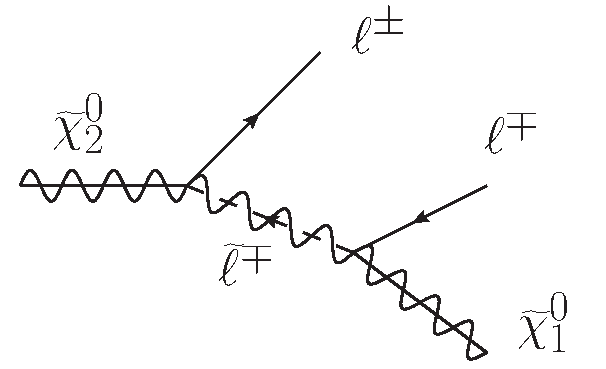
\includegraphics[width=\textwidth]{plots/THEO/FeynmanGraph_slepton.pdf}
\end{minipage}
\begin{minipage}[t]{0.49\textwidth}
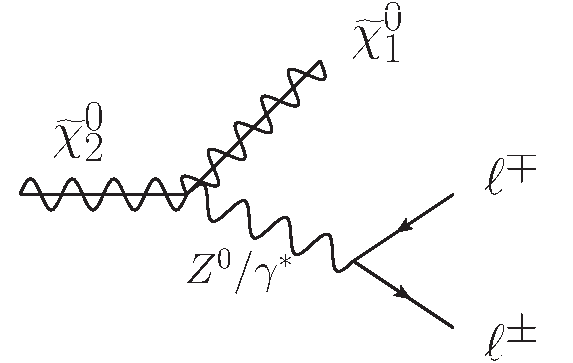
\includegraphics[width=\textwidth]{plots/THEO/FeynmanGraph_Z_decay.pdf}
\end{minipage}
\caption{Graphs for the decays of \secondchi into $\firstchi\ell^+\ell^-$ via an intermediate slepton (left) and off- or on-shell Z boson. Graphs by Christian Schomakers.}
\label{fig:edgeFeyn}
\end{figure}

The mass difference between the two neutralinos sets an upper bound on the invariant mass of the dilepton system \mll and its distribution exhibits an characteristic edge structure. The endpoint of this edge is defined by the signal kinematics.  If the \secondchi decays via an off-shell Z boson, it is simply given by the mass difference itself:
\begin{equation}
\mlledge = m_{\secondchi} - m_{\firstchi}.
\end{equation}
If the decay is mediated via a slepton, this is modified by the slepton mass $m_{\tilde{\ell}}$
\begin{equation}
\mlledge = \sqrt{\frac{(m_{\secondchi}^2-m_{\tilde{\ell}}^2)(m_{\tilde{\ell}}^2-m_{\firstchi}^2)}{m_{\tilde{\ell}}^2}}. 
\end{equation}
For decays via and on-shell Z boson, \mll will be consistent with the Z boson mass and no edge structure is present. The exact shape of the edge is also determined by the decays. For intermediate Z bosons, it will be peaked towards the Z boson peak for \mlledge below the Z peak. For \mlledge on and above the Z boson peak, the decays via and on-shell Z boson dominate and there is no edge. Decays via an intermediate sleptons lead to triangular edge shapes, but the actual shape depends on model parameters, as for example negative interference between the decay channels via slepton and Z boson can occur. Examples are given in the next section.
\subsubsection{Simplified models}
\label{sec:models}
As benchmark scenarios for these signatures, two ``simplified models'' are used that have been developed for this purpose by Christian Schomakers in the context of his master thesis~\cite{Schomakers:2014zza}. In this kind of models, only the subset of sparticles relevant to the studied signature is assumed to be accessible at LHC energies. Also, the branching fractions of the sparticle decays are chosen to produce the desired signature and are often set to 100\%.  

Both models consider the pair production of bottom squarks. They decay into a bottom quark and a \secondchi with a branching fraction of 100\%. The decays of the \secondchi differ between the two models. The Feynman graphs of both models are shown in Figure~\ref{fig:sigFeyn}.

\begin{figure}[htbp]
\centering
\begin{minipage}[t]{0.49\textwidth}
  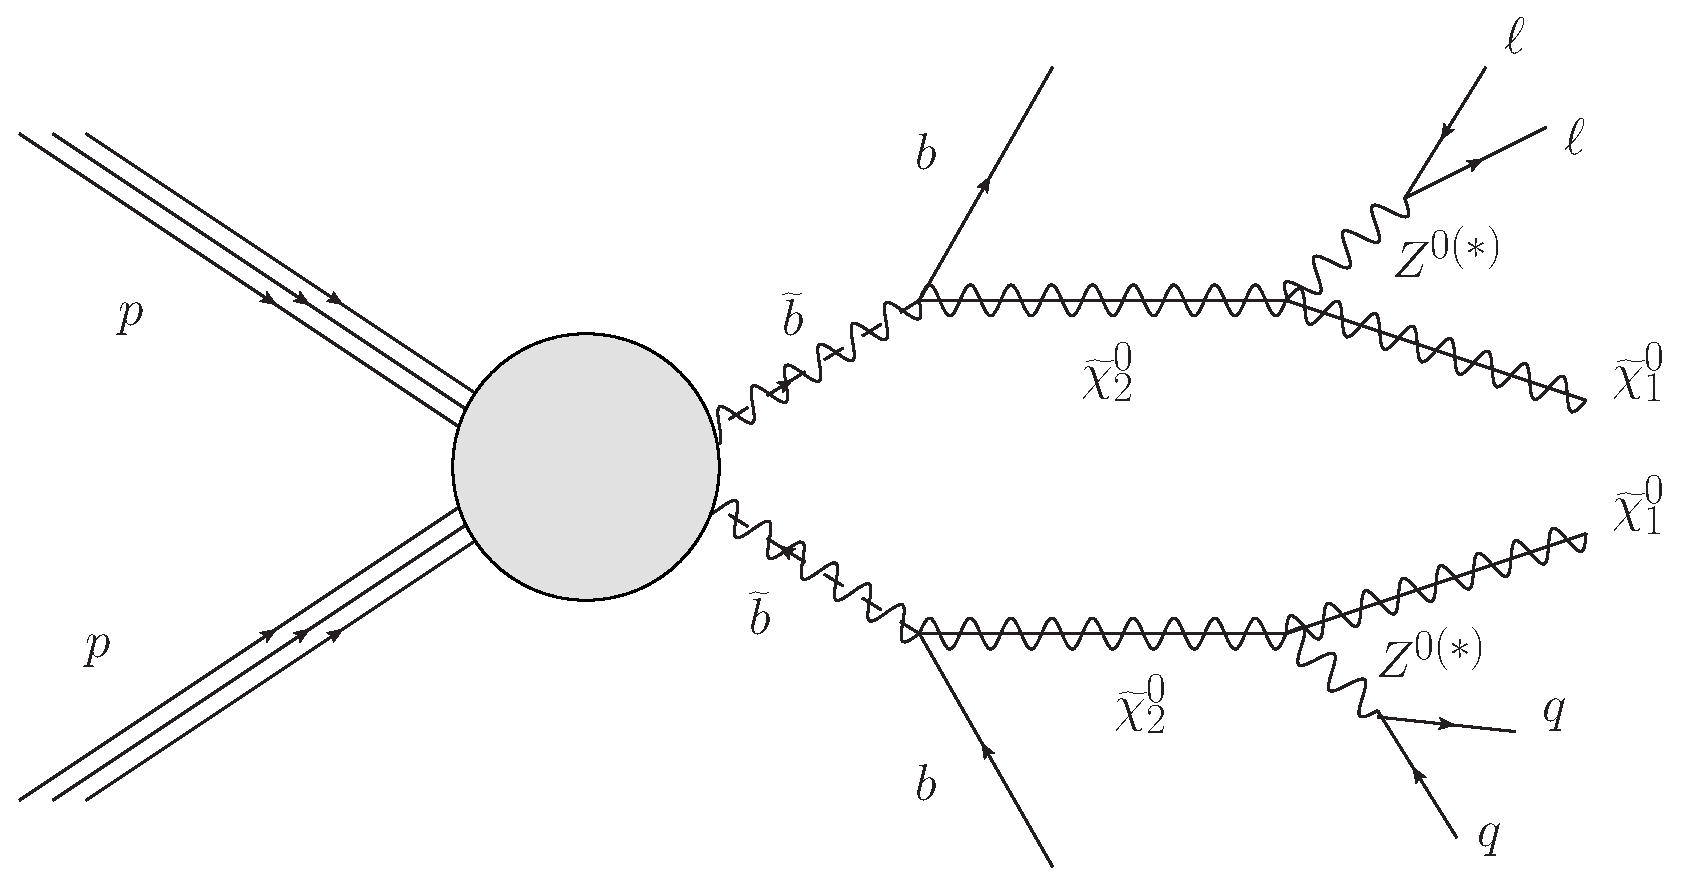
\includegraphics[width=\textwidth]{plots/THEO/Feynman_graph_T6bblledge.pdf}
\end{minipage}
\begin{minipage}[t]{0.49\textwidth}
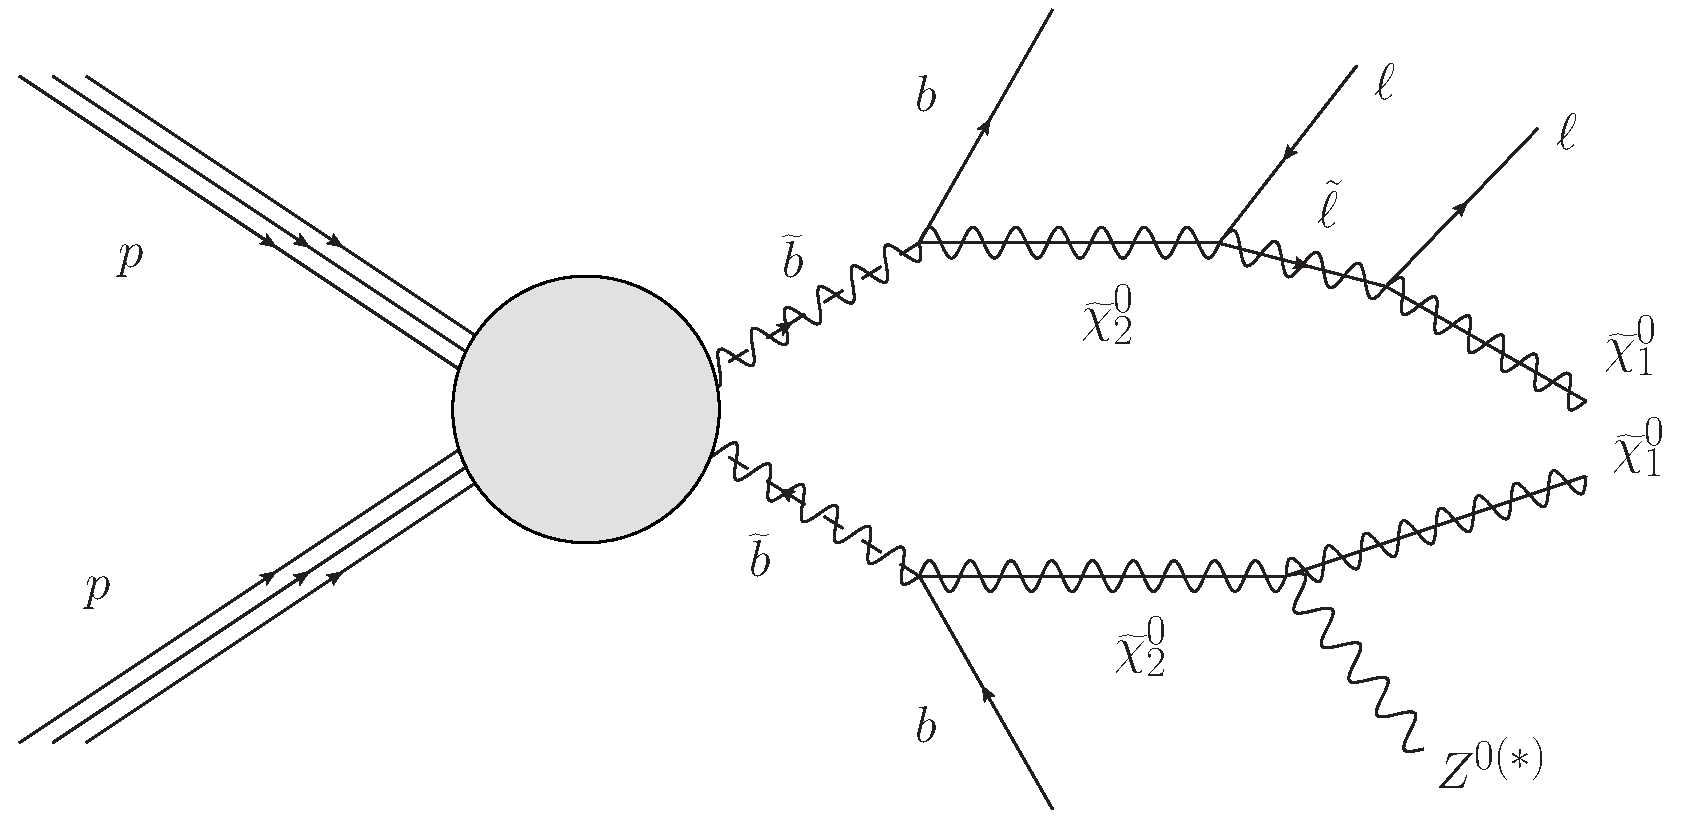
\includegraphics[width=\textwidth]{plots/THEO/Feynman_graph_T6bbslepton.pdf}
\end{minipage}
\caption{Feynman graphs for the fixed-edge (left) and slepton-edge (right) model~\cite{Khachatryan:2015lwa}.}
\label{fig:sigFeyn}
\end{figure}

 In the ``fixed-edge'' model, it decays into an off-shell Z boson and a \firstchi in 100\% of the cases. The Z boson decays with its SM branching ratios, producing light leptons in about 7\% of the cases. The $m_{\sbottom}$-$m_{\secondchi}$-plane is scanned, varying the masses of the two particles in steps of 25\GeV. The mass of the \firstchi is fixed to be 70\GeV below that of the \secondchi to produce an edge in the \mll spectrum at this value.

As a mass difference between the two neutralinos larger than the Z boson mass would only result in the production of on-shell Z bosons in this model, the ``slepton-edge'' model introduces selectrons and smuons as additional new particles. The mass of these sleptons is assumed to be degenerate and set to lie halfway between the two neutralinos: $m_{\slepton} = m_{\firstchi} + 0.5(m_{\secondchi}-m_{\firstchi})$. The branching fractions of the \secondchi are chosen such that the decay in an off- or on-shell Z boson or a slepton and a lepton occur with 50\% probability each. The Z boson again decays according to its SM branching fraction while the slepton always decays into a lepton and the \firstchi. Again the $m_{\sbottom}$-$m_{\secondchi}$-plane is scanned in steps of 25\GeV, while the $m_{\firstchi}$ is set to be 100\GeV, allowing for edges in the \mll spectrum also above the Z boson mass. 
The signal simulation is normalized to theory cross sections calculated at NLO in $\alpha_s$, including the leading logarithmic contributions of the next higher order~\cite{bib-nlo-nll-01,bib-nlo-nll-02,bib-nlo-nll-03,bib-nlo-nll-04,bib-nlo-nll-05,ref:xsec}.

Figure~\ref{fig:SUSYMasses} illustrates the \mll distributions for three example points. The two examples from the slepton-edge model are roughly triangular in shape while the one from the fixed-edge model is peaked toward the Z boson peak as in this model the decay is mediated by an off-shell Z boson. Contributions outside of the edges are caused by events with more than two leptons where the wrong combination has been chosen. In addition to the generated distribution the one reconstructed by a simulation of the CMS detector is shown, illustrating the good detector resolution for lepton pairs.
\begin{figure}
\centering
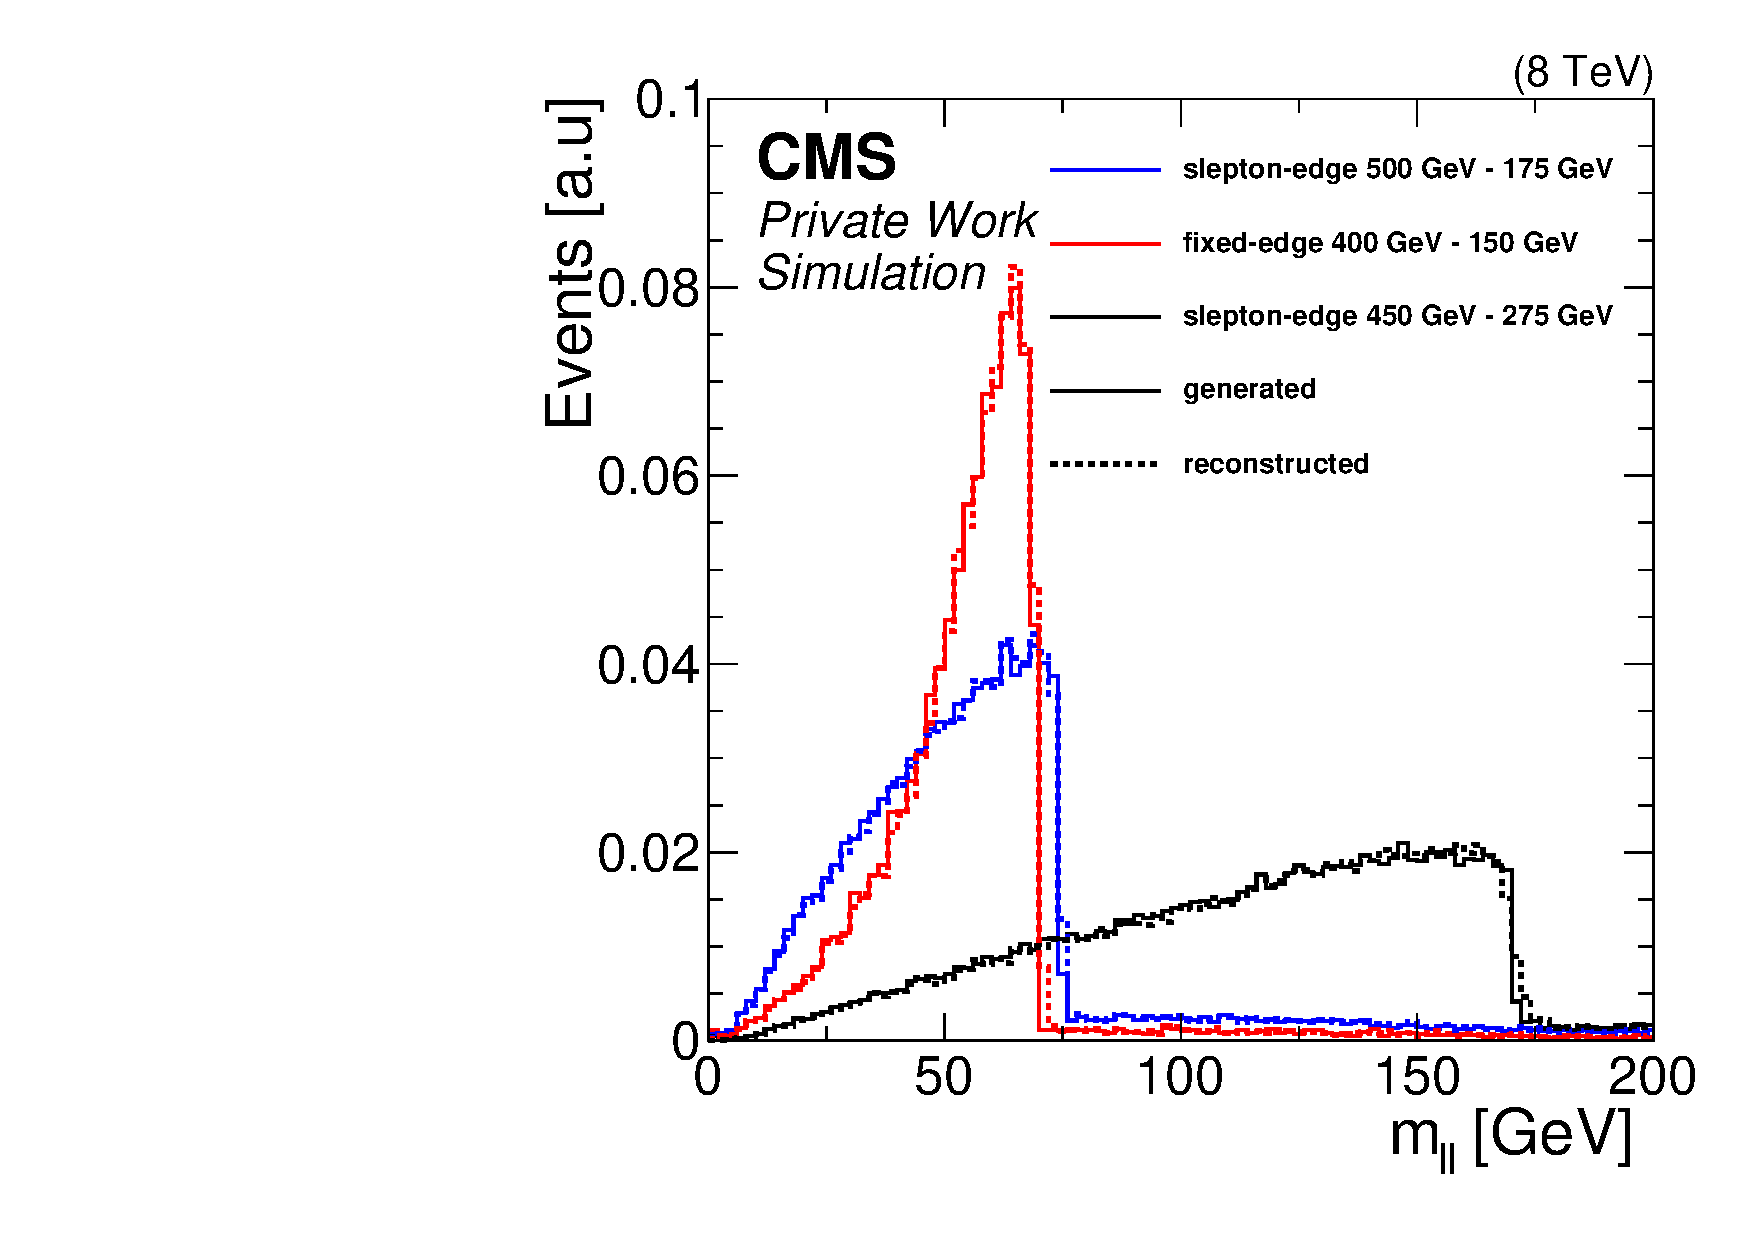
\includegraphics[scale=0.3]{plots/THEO/SUSY_masses.pdf}
\caption{Distribution of \mll for one signal point of the fixed-edge model and two of the slepton-edge model, illustrating different edge positions and shapes. The masses given are those of the \sbottom and \secondchi, respectively. Shown are the generated distributions as solid lines and the reconstructed ones as dashed lines.}
\label{fig:SUSYMasses}
\end{figure}

     